\chapter{Multi-port Deterministic Suffix-Reading Automata}
\label{sec:intro}

The preceding chapters developed the theory of Deterministic Suffix-reading Automata (DSAs) as a powerful tool for the succinct specification of \emph{sequential}, pattern-based systems. However, modern software and hardware systems are rarely monolithic; they are typically composed of multiple interacting components that operate concurrently. This chapter pivots our investigation from the sequential to the concurrent domain, addressing the new set of challenges that arise when specifying the behavior of such systems.

A primary obstacle in modeling concurrent systems with sequential automata is the `interleaving explosion'. To capture all possible behaviors, a model must typically account for every possible ordering of asynchronous events from different components. For example, a requirement that a car can only start after receiving signals for the key in ignition ($K$), brake pressed ($B$), and transmission in park ($P$)—in any order—would force a standard DSA to explicitly enumerate all $3! = 6$ permutations of these events on transition labels. As the number of concurrent components grows, this approach becomes combinatorially infeasible and defeats the purpose of DSA as a concise specification~\cite{DBLP:journals/corr/abs-2410-22761}.





  \begin{figure}
  \centering
  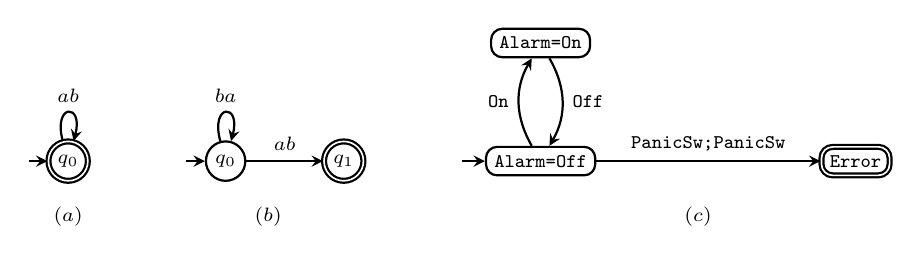
\begin{tikzpicture}[state/.style={circle, inner sep=2pt, draw, thick}]
    \begin{scope}[every node/.style={state}]
      \node [double] (0) at (0,0) {\scriptsize $q_0$};
    \end{scope}
    \begin{scope}[->, >=stealth, thick]
      \draw (-0.5, 0) to (0);
      \draw (0) to [loop above] node {\scriptsize $ab$} (0);
    \end{scope}
    \node at (0, -0.7) {\scriptsize $(a)$};

    \begin{scope}[xshift=2cm]
      \begin{scope}[every node/.style={state}]
        \node (0) at (0,0) {\scriptsize $q_0$};
        \node [double] (1) at (1.5, 0) {\scriptsize $q_1$};
      \end{scope}
      \begin{scope}[->, >=stealth, thick]
        \draw (-0.5, 0) to (0);
        \draw (0) to [loop above] node  {\scriptsize $ba$} (0);
        \draw (0) to node [above] {\scriptsize $ab$} (1);
      \end{scope}
      \node at (0.54, -0.7) {\scriptsize $(b)$};
    \end{scope}

      \begin{scope}[xshift=6cm]
        \begin{scope}
          \node [rectangle, rounded corners, draw, inner sep=3pt, thick] (0) at (0,0) {\scriptsize \texttt{Alarm=Off}};
          \node [rectangle, rounded corners, draw, inner sep=3pt, thick] (1) at (0,1.5) {\scriptsize \texttt{Alarm=On}};
          \node [rectangle, rounded corners, draw, inner sep=3pt, thick, double] (2) at (4, 0) {\scriptsize \texttt{Error}};
        \end{scope}

        \begin{scope}[->, >=stealth, thick]
          \draw (-1,0) to (0);
          \draw (0) to [bend left] node [left] {\scriptsize \texttt{On}} (1);
          \draw (1) to [bend left] node [right] {\scriptsize \texttt{Off}} (0);
          \draw (0) to node [above] {\scriptsize \texttt{PanicSw;PanicSw}} (2);
        \end{scope}
        \node at (2, -0.7) {\scriptsize $(c)$};
      \end{scope}
    
  \end{tikzpicture}
  \caption{Examples of Deterministic Suffix-reading Automata (DSA)}
  \label{fig:dsa-examples}
  \end{figure}






  In Figure~\ref{fig:dsa-examples}(a), the DSA accepts all words that end with $ab$, for instance $bab, bbab, babaab$, etc. The transition $q_0 \xra{ab} q_0$ is fired as soon as a word ending with $ab$ is seen after reaching $q_0$. For instance, on the word $babaab$, the transition is first triggered on the prefix $bab$ since this is the first time $ab$ appears as suffix; once the transition is triggered, the prefix $bab$ has been consumed, and now we are left with $aab$; on reading $aab$ fully, the transition $q_0 \xra{ab} q_0$ is triggered again.  In Figure~\ref{fig:dsa-examples}(b), we can view the state $q_0$ as tracking two suffixes $ba$ and $ab$. When $ba$ is seen before $ab$, the self-loop is triggered; otherwise when $ab$ is seen first, the transition to $q_1$ is taken. For example, on word $bbab$, the automaton starts at $q_0$, and on $bba$ it fires $q_0 \xra{ba} q_0$ (since $ba$ is a suffix of $bba$), then reads $b$ and remains there. %Since $q_0$ is non-accepting, the word is rejected. 
  However, on $bbaab$, the run loops on $bba$ back to $q_0$, and then reads the next $ab$ to reach $q_1$, and accept. The final example Figure~\ref{fig:dsa-examples}(c) is a \emph{suffix-based specification} of a part of an automotive software: when the alarm is off, and the panic switch is pressed twice within one second, flag an error. Here, we assume there is a symbol \texttt{tick} to denote the elapse of $1$ unit of time. So, on a word \texttt{tick}; \texttt{On}; \texttt{tick}; \texttt{Off}; \texttt{PanicSw}; \texttt{PanicSw}, an error should be flagged (we have added a separator symbol ; just for clarity). This specification is succinctly represented by the DSA in Figure~\ref{fig:dsa-examples}(c).

   Since transitions in a DSA wait for specific patterns to appear, DSAs are able to represent suffix-based specifications succinctly. When we consider systems with multiple components (which we call ports), the requirements can talk about different combinations of inputs. Here are two examples. 

   \begin{figure}
   \centering
   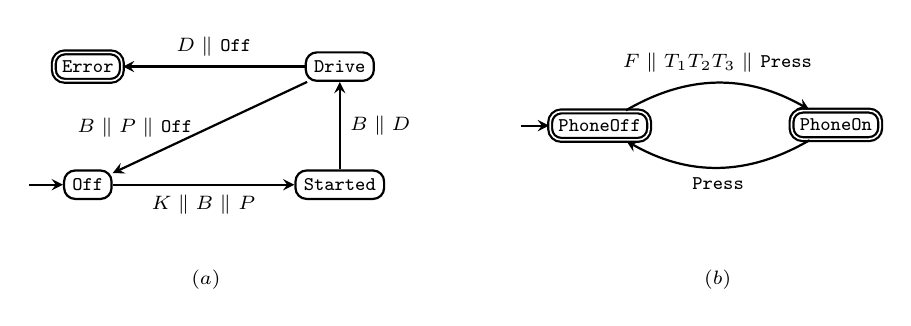
\begin{tikzpicture}
      \begin{scope}[every node/.style={rectangle, rounded corners, draw, inner sep=3pt, thick}]
        \node (0) at (0,0) {\scriptsize \texttt{Off}};
        \node [double] (1) at (0,1.5) {\scriptsize \texttt{Error}};
        \node (2) at (3.2,0) {\scriptsize \texttt{Started}};
        \node (3) at (3.2,1.5) {\scriptsize \texttt{Drive}};
      
      \end{scope}

      \begin{scope}[->,>=stealth, thick, auto]
        \draw (-0.75,0) to (0);
        %\draw (0) to [bend left] node [left] {\scriptsize \texttt{On}} (1);
        %\draw (1) to [bend left] node [right] {\scriptsize \texttt{Off}} (0);
        \draw (0) to node [below] {\scriptsize $K \parallel B \parallel$ $P$} (2);
        \draw (2) to node [right] {\scriptsize $B \parallel D$ } (3);
        \draw (3) to node [left] {\scriptsize $B \parallel P \parallel$ \texttt{Off}$~$} (0); 
        \draw (3) to node [above] {\scriptsize $D \parallel$ \texttt{Off}} (1);
      \end{scope}

      \node at (1.5, -1.2) {\scriptsize $(a)$};

      \begin{scope}[xshift=6.5cm]
        \begin{scope}[every node/.style={rectangle, rounded corners, draw, inner sep=3pt, thick}]
          \node [double] (0) at (0,0.75) {\scriptsize \texttt{PhoneOff}};
          \node [double] (1) at (3,0.76) {\scriptsize \texttt{PhoneOn}};
        \end{scope}

        \begin{scope}[->,>=stealth, thick, auto]
          \draw (-1,0.75) to (0);
          \draw (0) to [bend left] node {\scriptsize $F \parallel T_1 T_2 T_3 \parallel$ \texttt{Press}} (1);
          \draw (1) to [bend left] node {\scriptsize \texttt{Press}} (0);
        \end{scope}

        \node at (1.5, -1.2) {\scriptsize $(b)$};


      \end{scope}
   \end{tikzpicture}
   \caption{Concurrent suffix-based specifications as multi-port DSAs}
   \label{fig:mdsa-examples}
   \end{figure}
   \paragraph*{Car Security System.} For a car to start, you need: key in ignition ($K$), brake pedal pressed ($B$), and transmission in park ($P$). The actions $K$, $P$ and $B$ can occur in any order. A DSA would need to represent this requirement using all $6$ permutations. Instead, we assume an alphabet that is distributed across different \emph{ports} -- ignition, brake pedal, transmission, and denote the concurrent actions as $K \parallel B \parallel P$. Here are some requirements of a car security system. Figure~\ref{fig:mdsa-examples}(a) illustrates the enriched DSA.

   \begin{itemize}
   \item When the brake pedal is pressed ($B$), transmission is in park $(P)$ and key is in ignition ($K$), the car can be started.
   \item If the brake pedal is pressed ($B$) and the transmission is moved to drive ($D$), the car goes to the drive mode.
   \item When the brake pedal is pressed ($B$), transmission is in park ($P$), and the ignition becomes off ($\mathtt{Off}$), the car is switched off. If ignition is switched off when brake is not pressed or when transmission is in drive/reverse, signal an error.
   \end{itemize}

  
   \paragraph*{Smartphone Lock Pattern.} 
   Figure~\ref{fig:mdsa-examples}(b) represents the enriched DSA modeling the requirements below for a smartphone lock.

   \begin{itemize}
   \item When the button is pressed ($\mathtt{Press}$), fingerprint verified $(F)$ and a correct pattern is received $(T_1 T_2 T_3)$, then the phone is switched on.
   \item If the phone is on, and the button is pressed, the phone is switched off.  
   \end{itemize}
   
  To the best of our knowledge, no automaton model can succinctly represent the combination of suffix-based patterns across a concurrent system. Incorporating concurrency into the specification is paramount when requirements talk about different components of a concurrent system. 




  

This challenge motivates the extension of our suffix-reading paradigm. The goal is to create a formalism that can directly express the logical intent of concurrent rules, such as `$K \parallel B \parallel P$', thereby abstracting away the details of interleaving. This requires a new model, which we call the `Multi-port Deterministic Suffix-reading Automaton (mDSA)'. The core idea is to partition the alphabet across multiple "ports" and introduce a parallel composition operator, `$\parallel$', into the transition syntax.

However, simply adding a new operator is a trivial syntactic change; the deep technical challenge lies in defining a formal operational semantics that is both theoretically sound and intuitively correct for real-world scenarios. This chapter grapples with a fundamental semantic dilemma: should the history of events be "consumed" after a transition, or should it persist as context? The \emph{Car Security System} example requires persistent context (the brake may need to remain pressed for a future action), while the \emph{Smartphone Lock} example requires detecting a "fresh" button press to avoid infinite loops on old data.

To resolve this, we will show that a novel, tape-based semantics is required. This work is further motivated by practical needs in Model Based Testing (MBT)~\cite{10.1145/1353673.1353681, 10.1002/stvr.456}. Industrial specification notations like Expressive Decision Tables (EDTs)~\cite{DBLP:conf/date/VenkateshSKA14} are used for test generation~\cite{DBLP:conf/enase/VenkateshSZA15a, DBLP:conf/icst/AgrawalVSZV20} and already employ a form of concurrent, suffix-based logic, but have historically lacked a rigorous formal semantics. A key contribution of this work is to provide such a semantics via the mDSA framework. This chapter will therefore define the mDSA model and its semantics, while subsequent chapters will extend it with outputs to fully capture and analyze notations like EDTs.

%marker





  %Finite state automata are all-pervasive, adopting different roles in different contexts. We focus on the role of automata as \emph{formal models of system requirements} and their subsequent application in Model Based Testing (MBT). MBT is a paradigm in formal methods where the requirements of a system under test (SUT) are first converted to a formal model. This formal model is then used to automatically generate test cases for the SUT. There are many MBT tools (see \cite{10.1145/1353673.1353681,10.1002/stvr.456} for a survey) and in several of them, the formal model is given by some extension of finite automata. 

  %Converting requirements to a Deterministic Finite Automaton (DFA) or a Non-deterministic Finite Automaton (NFA) is often cumbersome. This is because DFAs and NFAs describe low level computations which reason about individual actions. There are various ways in which automata can be made consise. In Generalized Automata~\cite{DBLP:books/lib/Eilenberg76,giammarresi1999deterministic}, transitions contain words instead of single actions. A transition $q \xra{abb} q'$ is fired from $q$ if the word $abb$ is seen after the automaton reaches $q$. Therefore, requirements which depend on an exact sequence of actions can be represented using generalized automata more concisely. A natural extension is to allow for regular expressions in transitions, resulting in the model of Expression Automata~\cite{10.1007/978-3-540-30500-2_15} and its deterministic variant. Deterministic Expression Automata (DEA) impose restrictions on the regular expressions that can be used: they should result in a prefix-free language, and moreover, every pair of regular expressions out of state is language disjoint. This results in DEA recognizing a subset of regular languages. On the other hand, in (non-deterministic) Expression Automata, the transitions are so powerful that the states have almost no meaning: the entire automaton can be reduced to a single state and a single transition labeled by the regular expression representing the language. For languages leading to big automata, the corresponding regular expression can be complicated and incomprehensible. The goal is to hit a sweet spot where the transition labels are not too complicated, and at the same time there are fewer states than a DFA. 

   

  %Deterministic suffix-reading automata (DSAs)~\cite{DBLP:journals/corr/abs-2410-22761} are a recently introduced automaton model for regular languages. Transitions are  labeled with words (as in a generalized automaton), however, the semantics is different. A transition $(q, abb, q')$ is fired from $q$ if a word \emph{ending} with the suffix $abb$ is seen. When there are multiple transitions out of a state, the first transition that matches is fired. Figure~\ref{fig:dsa-examples} gives some examples of DSAs.




  
  %\subsubsection*{Contributions.} 
  The goal of this chapter is to investigate the
  addition of a parallel operator $\parallel$, into the
  transition syntax of DSAs. %We call the resulting model as \emph{multi-port DSAs}, where the alphabet is distributed (partitioned) across multiple ports.
  The challenge lies in describing an operational semantics that matches with
  our intentions. As our first technical contribution, we provide a formal
  operational semantics for multi-port DSAs, or mDSAs.
  
  %Next, we include the feature to produce outputs on transitions, giving us mDSA-with-outputs. When the produced outputs also influence suffix-based input conditions, the behaviours become more complex. In fact, we then show that state reachability for mDSA-with-outputs is $\PSPACE$-complete. When there are no outputs, reachability is simply linear in the input size.  

  %As our next contribution, we apply the mDSA framework to provide a formal semantics for Expressive Decision Tables (EDTs), a notation introduced by \cite{DBLP:conf/date/VenkateshSKA14} to incorporate both state-based and stream-based requirements in one convenient tabular form. The EDT notation has been successfully deployed in many industrial projects. In \cite{DBLP:conf/date/VenkateshSKA14} it has also been observed that the time and effort involved in writing EDT specifications was considerably low compared to other formalisms like  Statecharts. Many test generation tools for EDT specifications have been developed: given an EDT, and a row, the tool can generate a sequence of input actions that can trigger the input-side conditions of the particular row~\cite{DBLP:conf/enase/VenkateshSZA15a,DBLP:conf/icst/AgrawalVSZV20}. 
  %Although EDTs have been used extensively for test generation, the notation does not yet have a formal operational semantics because of a complex interplay between concurrency and suffix-based rules. We close these gaps using the mDSA technology: we consider a fragment of the EDT notation, and map each EDT to an mDSA-with-outputs. This in turn gives an operational semantics for the EDT. Moreover, test generation for EDTs reduces to state reachability in mDSA-with-outputs. We also develop a prototype implementation for state reachability in mDSA-with-outputs, using which we generate test cases for an intricate EDT example. 
  

  


\paragraph*{Related work.}
Use of automata to model concurrent systems has been explored widely.
Esterel~\cite{DBLP:journals/scp/BerryG92} is a synchronous programming language
that provides a parallel composition operator. Harel's
Statecharts~\cite{DBLP:journals/scp/Harel87} also support parallel composition
of state transition systems. In both these languages, the reaction of a system
in response to inputs on each port can be specified separately, and the
different specifications can be composed using the parallel operator. A system
model can then refer to the states of each port's specification to model the
system behaviour. In mDSAs, we do not compose automata. Instead there is a single automaton, but the transitions include a parallel composition operator. More importantly, mDSA allows for suffix-based event triggers. %specifications are more succinct than Statecharts or Esterel specifications of System behaviours similar to the examples described in this
%paper. 

Petri nets~\cite{CAPetri}
have been studied extensively to model concurrent systems. In Petri nets, each
letter of each port's alphabet will have to be represented using a place, and
the places combined to model the system. There is no mechanism to include suffix-based triggers. %This will not be as succinct as an
%mDSA. 
The work that is closest to ours is Input/Output Partial Order
Automata (IOPOA)~\cite{10.5555/2391293.2391305}. In their work, transitions
execute non-atomically reacting to asynchronous inputs on several ports. The
main differences between IOPOA and mDSA: in mDSA transitions react
atomically, transition labels can be strings representing a suffix for each port and not just letters,
a,nd different transitions may trigger on the same string at a port. For example, in the mDSA in Figure~\ref{fig:mdsa-examples}(a), the transitions from $\mathtt{Off}$ to $\mathtt{Started}$ and $\mathtt{Started}$ to $\mathtt{Drive}$ can be taken on the same input $B$. In an IOPOA this will require two occurences of $B$. IOPOA was primarily designed to enable test generation, whereas the aim of mDSAs is succinct specification of requirements.

%\paragraph*{Structure of the paper.} %Section~\ref{sec:prelims} briefly recalls the syntax and semantics of Deterministic Suffix-reading Automata (DSA). 
%In Section~\ref{sec:multiport}, we extend DSA with the parallel operator, and in section~\ref{sec:multiport-outputs}, we add the feature to produce outputs. Finally in Section~\ref{sec:edt}, we describe the EDT notation and the translation from EDT to multi-port DSA with outputs. 





\section{Extending DSA to accommodate multiple ports}
\label{sec:multiport}

Consider a special kind of alphabet
$\Sigma = \langle \Sigma_1, \Sigma_2, \dots, \Sigma_k \rangle$ such
that $\Sigma_i \cap \Sigma_j = \emptyset$ for all $i, j \in
\{1, \dots, k\}$. We will call $\Sigma_i$ as the alphabet of \emph{port} $i$,
and $\Sigma$ as a \emph{multi-port} alphabet. For instance, in the \emph{Car Security System specification} of Section~\ref{sec:intro}, there are three ports: brake, transmission and ignition, with $\Sigma_{\mathsf{brake}} = \{B\}$, $\Sigma_{\mathtt{trm}} = \{ P, D\}$ and $\Sigma_{\mathtt{ig}} = \{ K, \mathtt{Off} \}$ respectively.  

We look at DFAs over such multi-port alphabets. Such DFAs model properties of systems 
that listen to inputs from different components and perform actions
based on them. Sometimes the order in which the system receives its
inputs from different ports is not relevant. For example, at a state
$s$, if the system receives $a$ from port 1 and $b$ from port 2, in any
order, then it has to go to state $t$.  A DFA would model this with
transitions: $s \xra{a} s_a \xra{b} t$ and $s \xra{b} s_b \xra{a}
t$. A DSA would contain two transitions $s \xra{ab, ba} t$ (and some
other transitions, if needed, to take care of $aa$, $bb$). To get a
more succinct notation we will use a $\parallel$ operator. We will
write $s \xra{a \parallel b} t$ to mean that at state $s$, when
both $a$ and $b$ are received, the automaton moves to $t$. When there
are several components, this notation leads to significant
succinctness, for instance $a_1 \parallel a_2 \cdots \parallel a_n$
stands for all the $n!$ permutations of $a_1$ to $a_n$. We will also
allow expressions of the form $a_1 a_2 \parallel b$, which stands for
the set of words $\{a_1 a_2 b, a_1 b a_2, b a_1 a_2\}$ which shuffles
$a_1a_2$ and $b$. Section~\ref{sec:intro} illustrates further examples of the use of $\parallel$ operator in Figure~\ref{fig:mdsa-examples}. We will now formalize this idea.  We begin with some notation.%

\paragraph*{Notation.} For a word $w \in \Sigma^*$, we write
$\proj{i}(w)$ for the projection of $w$ onto the set $\Sigma_i$. For
instance, if $\Sigma_1 = \{a_1, a_2\}, \Sigma_2 = \{b_1, b_2\}$ and
$w = a_1 b_1 a_2 a_1 b_2 b_2$, we have $\proj{1}(w) = a_1 a_2 a_1$ and
$\proj{2}(w) = b_1 b_2 b_2$.  
Notice that if for two words $w_1, w_2$ suppose $\proj{i}(w_1) = \proj{i}(w_2)$ for all ports $i$, then $w_1$ and $w_2$ have the same order of events within each port, but could have a different ordering between letters from different ports.% 


\subsection{Some challenges in extending to multiport}
\label{sec:challenges}

For a DSA, a configuration was given by $(q, w)$ where $q$ is the current state and $w$ is the word seen after reaching $q$. Moreover, if a transition matches, the DSA moves to a configuration $(q', \epsilon)$ by fully consuming the word seen so far. Now consider the car security system example (Figure~\ref{fig:mdsa-examples} (a)) . On receiving inputs $P;B;K$, the automaton moves to $\mathtt{Started}$ state.
If the brake remains pressed and the transmission is moved to park, we would like the car to go into the drive mode. Therefore, on the word $P;B;K;D$, the automaton should go to the $\mathtt{Drive}$ state. This intention is summarized below as what we require as the run of the automaton:
\begin{align*}
  \mathtt{Off} \quad \xra{P;B;K} \quad \mathtt{Started} \quad \xra{D} \quad \mathtt{Drive}
  \end{align*} 
 If we had consumed the prefix $P;B;K$ while moving to the $\mathtt{Started}$ state, then the transition $B \parallel D$ would not match anymore, since there is no $B$ after reaching $\mathtt{Started}$. What we really need is that: the last seen input in the brake port is $B$ and the last seen input in the transmission port is $D$. Therefore, one option is to simply not consume any letters and say that a transition $u_1 \parallel u_2 \parallel \cdots \parallel u_k$ matches a word $w$ if $u_i$ is a suffix of projection $\proj{i}(w)$. However, this creates other problems as we will now illustrate. 
 
 Consider the smartphone lock pattern specification (Figure~\ref{fig:mdsa-examples} (b)). On a word $F; T_1; T_2; T_3; \mathtt{Press}$, the phone is unlocked and the automaton goes to the $\mathtt{PhoneOn}$ state. At this state, there is an outgoing transition that listens to $\mathtt{Press}$. If we do not consume the word seen so far, the last seen input in the button port is still $\mathtt{Press}$, and hence the automaton would go back to the $\mathtt{PhoneOn}$ state without seeing additional inputs. In fact, this looping behaviour would continue forever, with no inputs seen. Therefore, for the outgoing transition $\mathtt{Press}$ in the $\mathtt{PhoneOn}$ state, the intention is that we need to receive a fresh signal $\mathtt{Press}$.  
 
 To summarize: on a transition match, we do not want to consume the word seen so far (car security specification example); but simply not consuming the word leads to problems (smartphone lock pattern example). In the following, we adopt an intermediate approach, where we mark the position $\theta$ in the word where the last transition matched. For a new transition $u_1 \parallel u_2 \parallel \cdots \parallel u_k$ to match, in addition to having each $u_i$ as a suffix of $\proj{i}(w)$, we require at least one $u_i$ to appear entirely after the marked position $\theta$. We include an additional condition that every $u_i$ appears either entirely to the left of $\theta$ or to the right of $\theta$ to account for such examples: 
 \begin{align*}
  s_0 \xra{c \parallel a} s_1 \xra{cc \parallel b}s_2
 \end{align*}
 Action $c$ can denote a \texttt{click}. So, the pattern $cc$ denotes a double click. On seeing $a; c$ the automaton moves to $s_1$. Now if the inputs received are $b; c$, we do not want the transition $cc \parallel b$ to match. Instead, we want two clicks and a $b$ after the last match. The condition that every pattern appears entirely after this match, or entirely before this match takes care of this situation.
 




\subsection{Multi-port DSAs: formal syntax and semantics} 

We first describe the formal syntax and then proceed to an operational semantics given by a labeled transition system.

\begin{definition}[Multi-port DSA] Let
  $\Sigma = \langle \Sigma_1, \Sigma_2, \dots, \Sigma_k \rangle$ be a
  multi-port alphabet. A \emph{multi-port (deterministic)
    suffix-reading automaton} (written mDSA in short) $\Aa$ is a
  tuple $(Q, \Sigma, q_0, \delta, F)$ where $Q$, $q_0$ and
  $F$ are a finite set of states, the initial state and a set of
  accept states, respectively. %$L = \{\lt_1, \lt_2, \dots, \lt_p\}$ denotes a set of tape heads. 
  The transition relation
  $\delta \incl Q \times \Sigma_1^* \times \Sigma_2^* \times \cdots
  \times \Sigma_k^* \times Q$: each transition is of the form
  $(q, (u_1 \parallel u_2 \parallel \cdots \parallel u_k), q')$ where
  $u_i \in \Sigma_i^*$ (not all of them can be $\epsilon$). 
  We assume there are only finitely many transitions. 
 \end{definition}%
Figure~\ref{fig:mdsa-examples} gives two mDSAs adhering to this syntax. 

 For the semantics, it is convenient to assume that there is a \emph{tape} on which the automaton writes all its inputs. Initially, the tape is $\epsilon$. Each time an input letter $a \in \Sigma$ is received, the automaton appends it to the right of the tape. 
 
 \paragraph*{Notation.} For a word $w = a_1 \dots a_{n}$, with $a_i \in \Sigma$, we write $w(i)$ to denote the letter $a_i$. We remark our convention that the indices of $w$ start from $1$ (and not $0$). The length of $w$, denoted as $|w|$, equals $n$ (the number of letters). For $j \in \{1, \dots, n\}$ we write $w[i, j]$ to denote the substring $a_i a_{i+1} \dots a_j$.

  \paragraph*{mDSA semantics.} A \emph{configuration} of an mDSA is given by $(q, w, \theta)$ where
  \begin{itemize}
  \item $q$ is the current state,
  \item $w$ is the word read so far, from the beginning
  \item $\theta \in \Nat$ marks a position in the word where the last match of a transition appeared.  
  \end{itemize} 
  We refer to the pair $(w, \theta)$ as the \emph{tape configuration}.
  
  The formal semantics of an mDSA $\Aa$ is given by a transition system $\Ss^\Aa = (S, S_0, \xra{}, S_F)$  over the configurations: the set of nodes $S$ is  the set of all configurations $(q, w, \theta)$ (notice that this set is infinite); the initial node $s_0$ is $(q_0, \epsilon, 0)$, also called \emph{the initial configuration}; $S_F$  is the set of \emph{accepting configurations} which are configurations $(q, w, \theta)$ where $q \in F$ and $\theta = |w|$ (signaling reaching an accepting state immediately after a match); to describe the transition relation $\xra{}$, we first explain when a transition label matches with a tape configuration. 

  \begin{definition}\label{def:match}
    We say that a transition label $(u_1 \parallel u_2 \parallel \cdots \parallel u_k)$ matches a tape configuration $(w, \theta)$ if:
    \begin{itemize}
      \item $u_i$ is a suffix of $\proj{i}(w)$ for all ports $i$,
      \item each $u_i$ appears entirely before or entirely after $\theta$: that is, $u_i$ is a subword of $w[1, \theta]$ or $w[\theta+1, |w|]$,
      \item at least one $u_i$ appears entirely after $\theta$.
    \end{itemize}
  \end{definition}

Let $\rho: (q, (u_1 \parallel u_2 \parallel \cdots \parallel u_k), q')$ be an outgoing transition from $q$. 
\begin{itemize}
\item In $\Ss^\Aa$, there is a following transition:
\begin{align*}
 (q, w, \theta) \xra[~u_1 \parallel u_2 \parallel \cdots \parallel u_k~]{a} (q', wa, \theta') \qquad \text{if}
\end{align*}
$(u_1 \parallel u_2 \parallel \cdots \parallel u_k)$ matches the tape configuration $(wa, \theta)$, and $\theta' = |wa|$ (tape head moves to the end of the tape).
\item There is a transition of the form:
\begin{align*}
  (q, w, \theta) \xra{a} (q, wa, \theta)
\end{align*}
if no transition out of $q$ matches the tape configuration $(wa, \theta)$. In this case, the tape head remains at its position.
\end{itemize} 

The transition relation $\xra{}$ of $\Ss^\Aa$ is a union over all $\xra[u_1 \parallel u_2 \parallel \cdots \parallel u_k]{a}$ and $\xra{a}$. 

 For all examples described in Section~\ref{sec:challenges}, the above semantics of transitions adheres to the required intention. 

\begin{remark}
We remark that the labeled transition system $\Ss^\Aa$ defined as above is non-deterministic, since multiple transitions can, in principle, be enabled at $(q, w, \theta)$ on seeing an $a$.  In order to make the automaton deterministic, a specific priority function can be added to resolve the non-determinism. If multiple transitions match at a configuration, the priority function is used to resolve the non-determinism. We did not explicitly add it to the syntax for technical simplicity.
\end{remark}

\begin{remark}
A DSA is an mDSA with a single port. To resolve non-determinism, DSAs employ the longest match criterion: among all strings that are a suffix, pick the one with the maximum length.
\end{remark}



%marker



This chapter successfully extended the suffix-reading paradigm from the sequential domain, as developed in the first part of this thesis, to the more complex realm of concurrent systems. We began by identifying the "interleaving explosion" as a primary barrier to the succinct modeling of concurrent specifications. In response, we introduced the \textit{Multi-port Suffix-reading Automaton} (mDSA), a model that uses a partitioned alphabet and a parallel composition operator to abstract away from specific event orderings.

The central contribution of this chapter was the development of a novel and robust operational semantics to handle the complex requirements of concurrent event-based logic. By introducing a tape-based configuration, $(q, w, \theta)$, which maintains the full history of inputs along with a marker for the last transition, we resolved the fundamental dilemma between needing persistent context for some conditions and fresh trigger events for others. We have thus established a formal, well-defined model capable of specifying complex, concurrent, and pattern-based system requirements in a concise and intuitive manner.

While the mDSA model presented here can recognize intricate combinations of inputs across multiple ports, many reactive systems must also \emph{produce outputs} or actions in response. In many practical specifications, an output generated by the system can immediately alter the state of the world, thereby influencing the conditions for subsequent transitions. To faithfully model this behavior and to provide a formal semantics for industrial notations like EDTs, our model requires one final extension. The next chapter will introduce this feature, defining the `mDSA-with-outputs' and exploring the computationally significant consequences of adding this feedback mechanism.






  
